\documentclass[12pt]{report}
\usepackage[
    a4paper,
    top=1cm,
    bottom=2cm,
    left=3cm,
    right=3cm,
    headheight=12pt,
    includehead,
    includefoot,
    heightrounded
]{geometry}
\usepackage{graphicx}
\usepackage[natbib=true, style=numeric, sorting=none]{biblatex}
\usepackage{fancyhdr}
\usepackage[dvipsnames, table]{xcolor}
\usepackage{parskip}
\usepackage{titlesec}
\usepackage{tocloft}
\usepackage{csquotes}
\usepackage{amsmath}
\usepackage[english]{babel}
\usepackage[style=iso, en-GB]{datetime2}
\usepackage{svg}
\usepackage{titling}
% \usepackage{hyperref}

\newcommand{\startappendix}[1]{
    \chapter{#1}
    \setcounter{page}{1}
    \pagestyle{fancy}
    \fancyhf[L,R,O,E]{}
    \fancyhead[C]{\textit{\title}}
    \fancyfoot[L]{Appendix}
    \fancyfoot[C]{\thechapter}
    \thispagestyle{fancy}
}

\titleformat{\chapter}[display]
    {\normalfont\LARGE\bfseries}
    {}
    {0pt}
    {}
\titlespacing{\chapter}
    {0pt}
    {0pt}
    {0pt}

\titleformat{\section}[display]
    {\normalfont\Large\bfseries}
    {}
    {0pt}
    {}
\titlespacing{\section}
    {0pt}
    {0pt}
    {0pt}

\titleformat{\subsection}[display]
    {\normalfont\large\bfseries}
    {}
    {0pt}
    {}
\titlespacing{\subsection}
    {0pt}
    {0pt}
    {0pt}

\titleformat{\subsubsection}[display]
    {\normalfont\normalsize\bfseries}
    {}
    {0pt}
    {}
\titlespacing{\subsubsection}
    {0pt}
    {0pt}
    {0pt}

\titleformat{\paragraph}[display]
    {\normalfont\small\bfseries}
    {}
    {0pt}
    {}
\titlespacing{\paragraph}
    {0pt}
    {4pt}
    {2pt}


\addbibresource{references.bib}

\def\course{EHD500}
\def\title{A remote SIM bank, a UE sink and a mediator -- Implementation of a utility for distributed coverage testing}
\def\swedishtitle{En fjärråtkomlig SIM-bank, en UE uppsamlare och en medlare -- Ett redskap för distribuerad täckningstestning}

\author{
    Hampus Avekvist
}

\def\examiner{Stanislav Belenki}
\def\advisor{
	Hanna Aknouche-Martinsson and Mikael Johansson,\\
	&Leissner Data AB
}
\def\swedishadvisor{
	Hanna Aknouche-Martinsson och Mikael Johansson,\\
	&Leissner Data AB
}

\def\keywords{
    5--10 words, separated by commas, describing the \\
    &contents of the report
}
\def\swedishkeywords{
    Här skrivs 5--10 ord, åtskilda med kommatecken, som \\
    &beskriver rapportens innehåll, ej ord från titeln
}


\begin{document}

\begin{titlepage}
    \thispagestyle{plain}
    \fancypagestyle{plain}{
        \renewcommand{\headrulewidth}{0pt}

        \fancyfoot[C]{}

        \fancyfoot[L]{
			\textbf{
				\vspace{-2cm}\\
				DEGREE PROJECT\\
				Computer Engineering\\
				Bachelor Level G2E, 15 hec
				\newline
				\newline
				Department of Engineering Science, University West, Sweden
			}
        }
    }

    \begin{minipage}{0.3\textwidth}
        \vspace{-1cm}
		
\includegraphics[width=\textwidth]{images/university-west-logo}
    \end{minipage}
    \hfill
    \begin{minipage}{0.4\textwidth}
        \vspace{-3cm}
        \begin{flushright}
		\textbf{\DTMsetstyle{iso}\today}
        \end{flushright}
    \end{minipage}

    \vspace{5cm}

    \Huge
	\textbf{\title}

    \Large
    \vspace{1cm}
	\textbf{\theauthor}
\end{titlepage}


\setcounter{secnumdepth}{0}
\pagenumbering{roman}

\begin{center}
    \large{\textbf{\textit{EXAMENSARBETE}}}

    \Large{\textbf{\swedishtitle}}
    {\rule{\textwidth}{0.8pt}}
    \vspace{6pt}
\end{center}

\section*{Sammanfattning}
Detta är en dokumentsida som skall sitta direkt efter titelsidan.
Den innehåller först och främst en sammanfattning av innehållet i
rapporten, och kompletteras med lämpliga uppgifter i rutan nedan.

Layouten på titel- och dokumentsidor får inte ändras, men sidorna
måste anpassas efter vilket program och ämne som arbetet tillhör
samt vilken utbildningsnivå som avses.

\vfill
\begin{table}[ht!]
    \centering
    \begin{tabular}{|l l|}
        \hline
        \textbf{Datum:} & \DTMsetstyle{iso}\today \\
        \textbf{Författare:} &\theauthor \\
        \textbf{Examinator:} &\examiner \\
        \textbf{Handledare:} &\swedishadvisor \\
        \textbf{Program:} &Datateknik, högskoleingenjör -- programmering och \\
                 &nätverksteknik, 180 hp \\
        \textbf{Huvudområde:} &Datateknik \\
        \textbf{Utbildningsnivå:} &Grundnivå \\
        \textbf{Kurskod:} &\course, 15 hp \\
        \textbf{Nyckelord:} &\swedishkeywords \\
        \textbf{Utgivare:} &Institutionen för ingenjörsvetenskap, Högskolan Väst \\
                  &461 86 Trollhättan \\
        \hline
    \end{tabular}
\end{table}
\newpage

\begin{center}
    \large{\textbf{\textit{DEGREE PROJECT}}}

    \Large{\textbf{\title}}
    {\rule{\textwidth}{0.8pt}}
    \vspace{6pt}
\end{center}

\section*{Summary}
Here the student is supposed to write a summary in English (even if
you write your thesis in Swedish). Hopefully, the student has
arrived at some interesting conclusions, so that the upper half of
this page will be stuffed with appropriate information.

\textbf{Note: you need to have an English title on top of this page}

\vfill
\begin{table}[ht!]
    \centering
    \begin{tabular}{|l l|}
        \hline
        \textbf{Date:} &\DTMsetstyle{en-GB}\today \\
        \textbf{Author:} &\theauthor \\
        \textbf{Examiner:} &\examiner \\
        \textbf{Advisor:} &\advisor \\
        \textbf{Programme:} &Computer Engineering -- programming and \\
                 &network technology, 180 hp \\
        \textbf{Main field of study:} &Computer Engineering \\
        \textbf{Education level:} &First cycle \\
        \textbf{Course code:} &\course, 15 HE credits \\
        \textbf{Keywords:} &\keywords \\
        \textbf{Publisher:} &Department of Engineering Science, University West \\
                  &SE-461 86 Trollhättan, Sweden \\
        \hline
    \end{tabular}
\end{table}



\pagestyle{fancy}
\fancyhf[L,R,O,E]{}
\fancyhead[C]{\textit{\title}}
\fancyfoot[C]{\thepage}

\fancypagestyle{plain}{%
    \fancyhf[L,R,O,E]{}
    \fancyhead[C]{\textit{\title}}
    \fancyfoot[C]{\thepage}
}

\thispagestyle{plain}

\section*{Preface}

I'd like to thank Leissner Data for the opportunity to implement a
novel technical system where much creativity had to be employed. I
would also like to thank them for the independence and trust to
work in my own way, allowing a thorough attempt at utilizing the
skills taught during the computer engineering program. I'm giving a
specific thanks to Peter Fässberg for the depths of knowledge he
provided during the design and discussions of the implementation.

TODO: Thank Hanna, Mikael and possibly others.


\setcounter{secnumdepth}{3}
\renewcommand*\contentsname{Table of contents}
\tableofcontents
\thispagestyle{fancy}


\chapter{Abbreviations}

\begin{table}[ht!]
    \centering
    \caption{Abbreviations}
    \label{tab:abbreviations}
    \begin{tabular}{|l|l|}
        \hline
        \rowcolor{lightgray}
        \textbf{Abbreviation} & \textbf{Description}            \\ \hline
        3GPP  & 3rd Generation Partnership Program              \\ \hline
        ADR   & Architectural decision record                   \\ \hline
        APDU  & Application Protocol Data Unit                  \\ \hline
        ATR   & Answer to Reset                                 \\ \hline
        ETSI  & European Telecommunications Standards Institute \\ \hline
        ICCID & Integrated Circuit Card Identifier              \\ \hline
        ISO   & International Organization for Standardization  \\ \hline
        ISP   & Internet Service Provider                       \\ \hline
        MVNE  & Mobile Virtual Network Enabler                  \\ \hline
        MVNO  & Mobile Virtual Network Operator                 \\ \hline
        PC/SC & Personal Computer / Smart Card                  \\ \hline
        PIN   & Personal Identification Number                  \\ \hline
        SIM   & Subscriber Identity Module                      \\ \hline
        SPN   & Service Provider Name                           \\ \hline
        TARA  & Threat assessment and risk analysis             \\ \hline
        USIM  & Universal Subscriber Identity Module            \\ \hline
    \end{tabular}
\end{table}


\titleformat{\chapter}[display]
    {\normalfont\LARGE\bfseries}
    {}
    {0pt}
    {\thechapter\ }

\titleformat{\section}[display]
    {\normalfont\Large\bfseries}
    {}
    {0pt}
    {\thesection\ }

\titleformat{\subsection}[display]
    {\normalfont\large\bfseries}
    {}
    {0pt}
    {\thesubsection\ }

\titleformat{\subsubsection}[display]
    {\normalfont\normalsize\bfseries}
    {}
    {0pt}
    {\thesubsubsection\ }


\newpage
\pagenumbering{arabic}

\chapter{Introduction}

Connectivity is essential for modern society. The ability to keep in
touch, share knowledge and collaborate remotely is growing evermore
important. A fundamental group of technologies and infrastructure
enables these facets, all categorized within the telecommunications
umbrella. Telecommunication businesses around the world compete to
provide the best service, while assisting one another to enable a
greater reach.

For a user of these technologies and infrastructure, identification
is required to ascertain the authenticity and capabilities that
should be provided. This is provided through a Subscriber Identity
Module (SIM) \cite{etsi-ts-131-102}, a type of smart card \cite{etsi-ts-102-221},
that stores encryption keys and application files utilized to verify
the subscriber in the telecommunications network. These SIM may have
varying support when roaming or if a device is 4G- or 5G-enabled.

Considering the varying support for SIM configurations in different
telecommunication networks, there is an interest for utilities that
can easily enable testing, configuration and manipulation of SIM:s,
preferably with user equipment (UE) in arbitrary locations and a bank
of SIM in an easily (though not unauthorized) accessible office space
that allows hot-swapping of the SIM connected to the differing UE.

The goal of this work is to develop said utilities that provide a
SIM bank, user equipment connectivity and a mediation service. The
mediation service enables pairing of SIM-to-UE with a logical
hot-swapping facility, rendering physical access to the SIM bank
only occasionally required rather than consistently.

The report starts off by introducing previous work in this sector,
formally introducing the problem and then provides necessary theory
and background information. The second chapter delves into the
methodology used in the design and implementation, alongside how
decisions were made and what material that was utilized. It also
shows the information collection process for relevant technical
specifications studied, used for the theory and background sections
in this chapter and the same information that guides the
implementation.

The third chapter addresses the results with a complete description
of the implementation alongside diagrams, measurement results from
the benchmarks and functionality tests described in \ref{sec:experimentation}.
In the fourth chapter, an analysis based on the implementation is
performed, addressing what could've been done differently and how
the tools, structure and method aided in the solution for the
problem at hand. Ethical considerations are provided and in the
fifth chapter conclusions are drawn.

\section{Background}

Leissner Data AB is a Swedish telecommunications firm from
Trollhättan founded in 1969 \cite{leissner-about}. The company
was not originally in telecommunications but pivoted to an 
Internet Service Provider (ISP) role in 1996 with the founding of
the sister company Götalandsnätet AB. In 2001 Leissner started
offering telecommunication systems and has since extended to mobile
platforms. These mobile platforms are, for example, complete
virtual mobile core infrastructure such as Packet Delivery Network
Gateways (PGW:s), Short Message Service Centers (SMSC:s) and Home
Subscriber Servers (HSS:s) \cite{leissner-mobile-core}.

After a partnership with Hi3G \cite{leissner-about}, Leissner
became a Mobile Virtual Network Enabler (MVNE) and in their
product catalogue, they sell SIM to the Mobile Virtual Network
Operators (MVNO). The aforementioned SIM:s is equipped with a
digital profile compatible with their systems. These digital
profiles are preset file structures and contents containing
information such as the International Mobile Subscriber Identifier
(IMSI), Service Provider Name (SPN) and encryption keys.

The digital profile may contain files that can be changed \cite{placeholder-source-for-smart-card-profiles},
e.g. the SPN or the Personal Identification Number (PIN) as well as
files that may not be changed, e.g. IMSI and Integrated Circuit
Card Identifier (ICCID). The design of the digital profiles is up
to the agreement between SIM supplier and the operator where which
files should be writeable or not can be decided.

Considering the aforementioned, a desire for a simplified test
platform arose. This test platform would allow hot-swapping of
SIM in a nearby location while having user equipment connecting
from a remote location, e.g. in another city or at a customer
office to test reliability and function of the mobile core
platform with different SIM profiles.

Functionality requested in such a platform include tracing of
application protocol data units (APDU:s) where the transmitted
APDU:s may be sniffed, or manipulation where transmitted APDU:s
are altered to e.g. transform one PIN into another or by changing
an SPN to something else. Reprogramming of SIM is another
requested capability which could replace existing software and
offer all SIM-related functionality inside a single system.

Lastly, support for other kinds of SIM than just physical in a
smart card reader is requested. This extends to virtual SIM in
a custom-developed runtime.

\section{Problem formulation}
\label{sec:problem-formulation}

The intention of this thesis is to implement a couple of technical
solutions addressing the requests from Leissner Data. The requests
can be dissolved into the following sections.

\subsection{Functionality}

Primary requested functionality is the ability to forward APDU:s
between a SIM and UE. This renders forwarding the initial problem
to solve and is dependent upon by secondary functionalities.
Tracing APDU:s and the ability to manipulate APDU:s extend the
forwarding functionality by either logging or changing the data.

Reprogrammability entails generating APDU:s from an alternative
source than from user equipment being sent directly to the SIM and
extends requirements to available functionality in a user
interface. This is out of scope for this project.

\subsection{Scalability}

Scalability in this case intends on providing an ability to add and
remove both SIM banks and UE from the system without configuration
changes in a central service. Both the SIM banks and the UE may be
in arbitrary locations.

\subsection{Security considerations}

The APDU:s may contain confidential information such as encryption
keys and identification numbers, normally not exposed due to the
locality of the SIM inside the UE but in the remote forwarding case
requiring hiding. Connectivity of the SIM bank and the UE to the
full system must also be handled in a secure way to not allow any
device to connect and get APDU delivered.

\subsection{Commercialization}

The nature of being able to test mobile core products on different
SIM profiles is not limited to only the developers of the products
themselves but also the business customers buying and operating the
products. Therefore, there is an interest in having a sellable
service and easily deployed devices a customer can order.

\subsection{Delimitations}

Manipulation of APDU:s, due to the added complexity in interface
design and time constraints will not be considered in this draft.
Similarly, the ability to reprogram SIM are out of scope for this
work as that relates to functionality not directly coupled with
the forwarding of APDU:s to and from a SIM and UE.

Only SIM will be considered in this implementation, excluding
general smart cards since the work is aimed at telecommunications.

\section{Previous work}

The primary inspiration and function description for this project
is Osmocom's remSIM project \cite{osmocom-remsim}. It is a
complete open source implementation of a SIM bank with forwarding
capabilities to user equipment. Osmocom provides a user manual,
open hardware and source code that is studied for this project's
implementation.

There are additional solutions in the field of SIM banks with
similar capabilities to the Osmocom remSIM and the proposed
solution described in this document. These solutions, however, are
proprietary \cite{polygator-sim-bank} complete solutions, usually
offering a cloud service they own \cite{placeholder-source-cloud-sim-bank}
not enabling the capabilities required for Leissner Data's purposes.
They may also restrict the communications protocol to the SIM bank
to a proprietary, undocumented protocol rendering implementation
difficult.

The existing solutions miss out on some of the requested
functionality and while they could be extended upon, Leissner Data
aims to develop their own solution to have full control of their
offering.

\section{Theory}

This section intends to elaborate on the necessary theory to
understand the utilization of SIM in the context of the
implementation and the related nomenclature.

\subsection{Nomenclature}

Definitions and descriptions of terminology commonly used in this
report are provided here. A word is explicitly stated if it has
a specific definition in regards to this document.

\subsubsection{User Equipment}

User Equipment (UE) is what in regular telecommunication contexts
may be used by a human, e.g. a mobile phone or wireless modems.
They may also be called mobile equipment or mobile stations.

\subsubsection{Subscriber Identity Module}

A SIM is a type of smart card utilized for the telecommunications sector
\cite{etsi-ts-131-102}. Historically it was called SIM during the prime of 2G,
but a later revision called Universal SIM (USIM) with 3G \cite{etsi-ts-131-102}
support was developed. USIM also enable 4G and 5G support given an
appropriate digital profile. While USIM may be the correct term, SIM
will be used in its place, though colloquially mean USIM.

A SIM is used to provide authentication capabilities by storing
encrypted keys and identification files within a telecommunications
application \cite{etsi-ts-131-102}. The SIM authenticates a
specific subscriber and their capabilities in a mobile network.

\subsubsection{Application Protocol Data Unit}

Application Protocol Data Units (APDU:s) are the application-level
communications protocol, residing on top of the transport layer of
a smart card and terminal interface \cite{etsi-ts-102-221}. These
may be file selections in the smart card, file reads, writes or
some other operation supported by the smart card \cite{etsi-ts-102-221}.

\subsubsection{SIM bank, SIM box or SIM farm}

A SIM bank is a device that provides connectivity to multiple SIM
simultaneously \cite{hyprms-sim-bank}. This may be used for
connecting to multiple operators or to have different SIM
configurations from a singular operator. One or more devices may
connect to the bank and choose which SIM to use, from which the
devices can act as user equipment.

The terms SIM bank, box and farm all refer to the same thing and
may be used interchangeably. Different sources use the different
phrases but SIM bank will used in this paper.

\subsubsection{SIM consumer}

SIM consumer in relation to this work is the device that receives
forwarded APDU:s from a remote SIM bank. It is also this device
that is connected to user equipment and therefore forwards the
received APDU:s to the UE.

\subsubsection{Mediator}

The mediator is in this paper the service that manages connections
between SIM:s in the SIM bank and ties them to a SIM consumer. It
manages Answer To Resets (ATR:s) for each SIM so user equipment
can identify the type of card upon connection establishment.
Alongside ATR:s, it forwards APDU:s to support tracing and
manipulation capabilities.

\subsection{Requirements engineering}

Requirements engineering is the craft of finding, defining,
validating and changing requirements for the solution of a problem \cite[111]{sommerville-software-engineering}.
Requirements grow and change alongside the lifecycle of a project
and requirements engineering is a formalization of how the process
works. Requirements can be separated into functional and
non-functional where functional requirements specify what a system
should do \cite[105-107]{sommerville-software-engineering} while
non-functional requirements specify peripheral qualities of the
system, such as implementation constraints, response time and
interface design \cite[107-111]{sommerville-software-engineering}.

The first step is elicitation, which includes gathering of
requirements from stakeholders, establishing the kind of
requirement, prioritizing and informally documenting said requirement \cite[112-120]{sommerville-software-engineering}.
Stakeholders \cite[103-104]{sommerville-software-engineering} are
people with legitimate interest in the system in question,
accounting for members of the development team, customers,
operational staff and others that are directly involved or affected
by the system. 

The second step is specification \cite[120-129]{sommerville-software-engineering}.
This entails writing formal or more technical specifications with
additional details relevant to the implementers but not all
stakeholders. Formalizations may take different appearances, as
shown in figure 4.11 in \cite[121]{sommerville-software-engineering}
where natural language, both in unstructured and structured form,
graphical notations and mathematical models are examples of
formalizations.

The third step is validation of the requirements \cite[129-130]{sommerville-software-engineering}.
This means testing the requirements for validity, consistency,
completeness, realism and verifiability. The step is vital to
ascertain the requirements are correct in the scope of the problem
at hand and that a proposed solution fulfilling the requirements also
solves the problem.

The last step is the change of requirements, specifically management of
changes \cite[130-134]{sommerville-software-engineering}. Letting
requirements change is important because new insights, knowledge and
changes in the surroundings spring up which affect the problem space.
Key points in managing changes is to provide traceability, which
entails tracking of relevant stakeholders for a requirement, how the
requirement has changed and why. The relationships between
requirements need also be tracked to identify peripheral changes when
a requirement is updated.

\chapter{Methodology}

\section{Literature study}

\subsection{Compilation of specifications}

To identify the capabilities and technologies usable for
implementation.

\subsection{Existing solutions and usage}

To provide examples of what has been done, how it may be used and
practical notes possibly missed from the specifications.

\section{Materials and equipment}
\label{sec:materials-and-equipment}

This section lists and elaborates on the equipment and material
used in the implementation.

\subsection{SIMtrace 2}

The SIMtrace 2 by Osmocom is an open hardware platform with open
source software \cite{simtrace}. It comes preloaded with SIM
tracing firmware called \verb|trace| \cite{simtrace-wiki} but
additional firmware for smart card emulation exists, provided by
Osmocom. This firmware is called \verb|cardem|
\cite{simtrace-wiki} and is used for communicating with user
equipment, sending APDU:s either constructed by software or
forwarded from a remotely accessed smart card. The hardware is
capable of tracing and emulating all kinds of ISO 7816
\cite{iso7816} smart cards when the T=0 protocol is used
\cite{simtrace-wiki} but the focus is on SIM.

\subsection{Raspberry Pi 4}

Two Raspberry Pi 4 units are used due to the ubiquity and
portability of the hardware platform. The main computer
requirements based on the proposed system are two Linux-based
devices with USB and IP network connectivity capabilities,
rendering most computer systems a viable choice where the choice
of Raspberry Pi is due to the small form factor, inexpensive
hardware and lower power drain, though none of those properties
are a requirement.

\subsection{Teltonika RUT200 v2.0}

The Teltonika RUT200 v2.0 is used as provisional user equipment
the SIMtrace 2 hardware running \verb|cardem| connects to, meaning
the receiver of forwarded APDU:s from a remotely accessed smart
card. The device provides 2G, 3G and 4G capabilities for mobile
network connectivity, authenticated to via the remotely accessed
smart card and has a WiFi and Ethernet interface allowing wired
and wireless connections and internet access, acting as a gateway
between the mobile network and the local network.

\subsection{Smart card readers, SIM, server and router}

Generic physical smart card readers are used for enabling access to
smart cards for the Raspberry Pi which will forward communications
from the smart card over IP to a destination device, e.g. a server
or a peer Raspberry Pi connected to a SIMtrace unit and user
equipment.

A server, virtual or not, is used as a central connectivity hub
enabling rerouting of SIM-to-UE communication to a either a
different UE or a different SIM. A basic router will be used to
provide IP network access for the Raspberry Pi and internet access
to the aforementioned connectivity hub.

\section{Prototype development}
\label{sec:prototype-development}

The initial development for explorative purposes is to create a
prototype \cite[62]{sommerville-software-engineering} \cite[56]{thomas-hunt-pragmatic-programmer} where ideas leading to
requirements, what to test for in a benchmarking and functionality
experiment which drives the decisions behind the final
implementation will be conducted. Requirements elicitation and
experimentation, described below, will use knowledge acquired in
the prototyping phase while also themselves provide additional
information that can sprout new concepts to initially implement in
the prototype before adding to the final implementation.

\section{Requirements elicitation}
\label{sec:requirements-elicitation}

Gather requirements, based on what the company wants to
accomplish and technical requirements based on specifications.

Functional and non-functional requirements, source from 
SEP book.

\section{Experimentation}
\label{sec:experimentation}

\section{Implementation}
\label{sec:implementation}

Test-driven development based on requirements and experience from
previous parts (prototype, experiment, requirements elicitation).

\subsection{Design process}

Documentation and architectural decision records (ADR)
\cite{adr, adr-github}.

\subsection{Testing}

Primarily for an explorative implementation of the requirements,
secondarily for remaining reliable.

\subsection{Benchmarking}

For identifying performance differentiations for code changes.
Tests may be benchmarked to see if it's running fast enough.

Reasons why performance may matter (unverified, find a source):
SIM and UE communication may require low latency, especially over
larger networks, considering they are otherwise usually
physically connected.

Most useful in relation to hot code paths and tight loops.

\subsection{Automated tooling}

Tools for documentation generation will be utilized, both for
automatic generation of changelogs that document available
functionality in an operational perspective but also tools that
generate software library documentation from code comments.
Examples of such tools are Doxygen \cite{doxygen} for software
library documentation generation and git cliff \cite{git-cliff} for
changelog generation.

To enable changelog generation, git cliff requires a consistent
format of git commits \cite{git-cliff} called Conventional Commits
\cite{conventional-commits}. This, using git cliff also enables
automatic version numbering \cite{git-cliff-bump-version} by
following the Semantic Versioning (SemVer) specification
\cite{semver}. If required, additional commit types will be created
and documented(in ADR:s?) with custom git parsers added to git
cliff \cite{git-cliff-tips-and-tricks}.

Automated testing.
gtest and gmock (if C++)

Automated benchmarking.
google microbenchmark (if C++)

\subsection{Delimitations}

The project is an initial implementation at Leissner Data for
verifying if it is viable to properly develop a product of this
kind. The intent is a technological exploration and will
therefore contain limited to no user testing. It will also avoid
testing graphical user interfaces (if necessary).

\section{Delimitations}

Only SIM cards are considered. No other smart cards will be used
at this time.

\chapter{Background/Theory}

\section{Nomenclature}

\paragraph{SIM - Subscriber Identity Module} A type of smart card
utilized for the telecommunications sector \cite{sim}. Historically
it was called SIM during the prime of 2G, but a later revision called
Universal SIM (USIM) with 3G \cite{usim} support surfaced. USIM also
enable 4G and 5G support given an appropriate digital profile. While
USIM may be the correct term, SIM will be used in its place, though
colloquially mean USIM.

SIM is used to provide authentication capabilities by storing
encrypted keys and identification files within a telecommunications
application \cite{sim-application}

\chapter{Results}

\chapter{Analysis/Discussion}

\chapter{Conclusions}

\section{Future work}

\subsection{Experimentation}
\label{sec:experimentation}

In tandem with prototyping, experiments testing multiple
implementations of the PC/SC \cite{pcsc} library in different
programming languages have been conducted. The experiments are to
guide technical decisions for what language to use depending on
which implementation that fulfills requirements for communications
with smart cards. Four languages were chosen, JavaScript (on
NodeJS) and Python, to compare two higher-level languages, as well
as C++ and Rust to compare two lower-level languages.

The experiments test the performance and ability to communicate
with multiple smart cards at the same time, when transmitting
multiple APDU:s in quick succession.

Idea: Elaborate on what will be tested and what measurements will
be taken and why.

Note: This section is a stub and needs additional information.

\subsection{Implementation}
\label{sec:implementation}

As already mentioned in chapter
\ref{sec:software-requirements-engineering}, tests will be used to
ensure requirements are being upheld. This leads swiftly into a
test-driven development approach
\cite[242-245]{sommerville-software-engineering} while system
design will be based around the non-functional requirements. The
process is iterative as mentioned in the previous sections and
shown in Fig.~\ref{fig:process-diagram}, where new findings in the
prototyping or experimentation stages drive changes in the main
implementation. The implementation step will equally drive a need
to return to the prototype, experimentation and a change of
requirements.

\begin{figure}[ht]
	\centering
	\includegraphics[width=0.5\textwidth]{images/process.mmd.png}
	\caption{The iterative development process. The dashed lines
	implies an optional order of execution}
	\label{fig:process-diagram}
\end{figure}

Throughout development, designs decisions are documented in
architectural decision records (ADR:s) \cite{adr, adr-github} that
contain related requirements. Said ADR:s will be structured,
describing what ideas were considered, which one was chosen and why
to allow historical transparency in the system design.



\titleformat{\chapter}[display]
    {\normalfont\LARGE\bfseries}
    {}
    {0pt}
    {}
\titlespacing*{\chapter}
    {0pt}
    {0pt}
    {0pt}

\pagenumbering{gobble}
\printbibliography[
    heading=bibintoc,
    title={References}
]
\thispagestyle{fancy}


\chapter{Figures}

\addcontentsline{toc}{chapter}{In larger reports, you may also
include a List of figures, List of tables, and maybe a List of
abbreviations}

\chapter{Abbreviations}

\begin{table}[ht!]
    \centering
    \caption{Abbreviations}
    \label{tab:abbreviations}
    \begin{tabular}{|l|l|}
        \hline
        \rowcolor{lightgray}
        \textbf{Abbreviation} & \textbf{Description}            \\ \hline
        3GPP  & 3rd Generation Partnership Program              \\ \hline
        ADR   & Architectural decision record                   \\ \hline
        APDU  & Application Protocol Data Unit                  \\ \hline
        ATR   & Answer to Reset                                 \\ \hline
        ETSI  & European Telecommunications Standards Institute \\ \hline
        ICCID & Integrated Circuit Card Identifier              \\ \hline
        ISO   & International Organization for Standardization  \\ \hline
        ISP   & Internet Service Provider                       \\ \hline
        MVNE  & Mobile Virtual Network Enabler                  \\ \hline
        MVNO  & Mobile Virtual Network Operator                 \\ \hline
        PC/SC & Personal Computer / Smart Card                  \\ \hline
        PIN   & Personal Identification Number                  \\ \hline
        SIM   & Subscriber Identity Module                      \\ \hline
        SPN   & Service Provider Name                           \\ \hline
        TARA  & Threat assessment and risk analysis             \\ \hline
        USIM  & Universal Subscriber Identity Module            \\ \hline
    \end{tabular}
\end{table}


\appendix

\titleformat{\chapter}[display]
{\normalfont\LARGE\bfseries}
{}
{0pt}
{\thechapter:\ }
\titlespacing*{\chapter}
{0pt}
{0pt}
{0pt}

\startappendix{Heading of second appendix}

\startappendix{Threat assessment and risk analysis}

\begin{figure}[ht!]
    \centering
    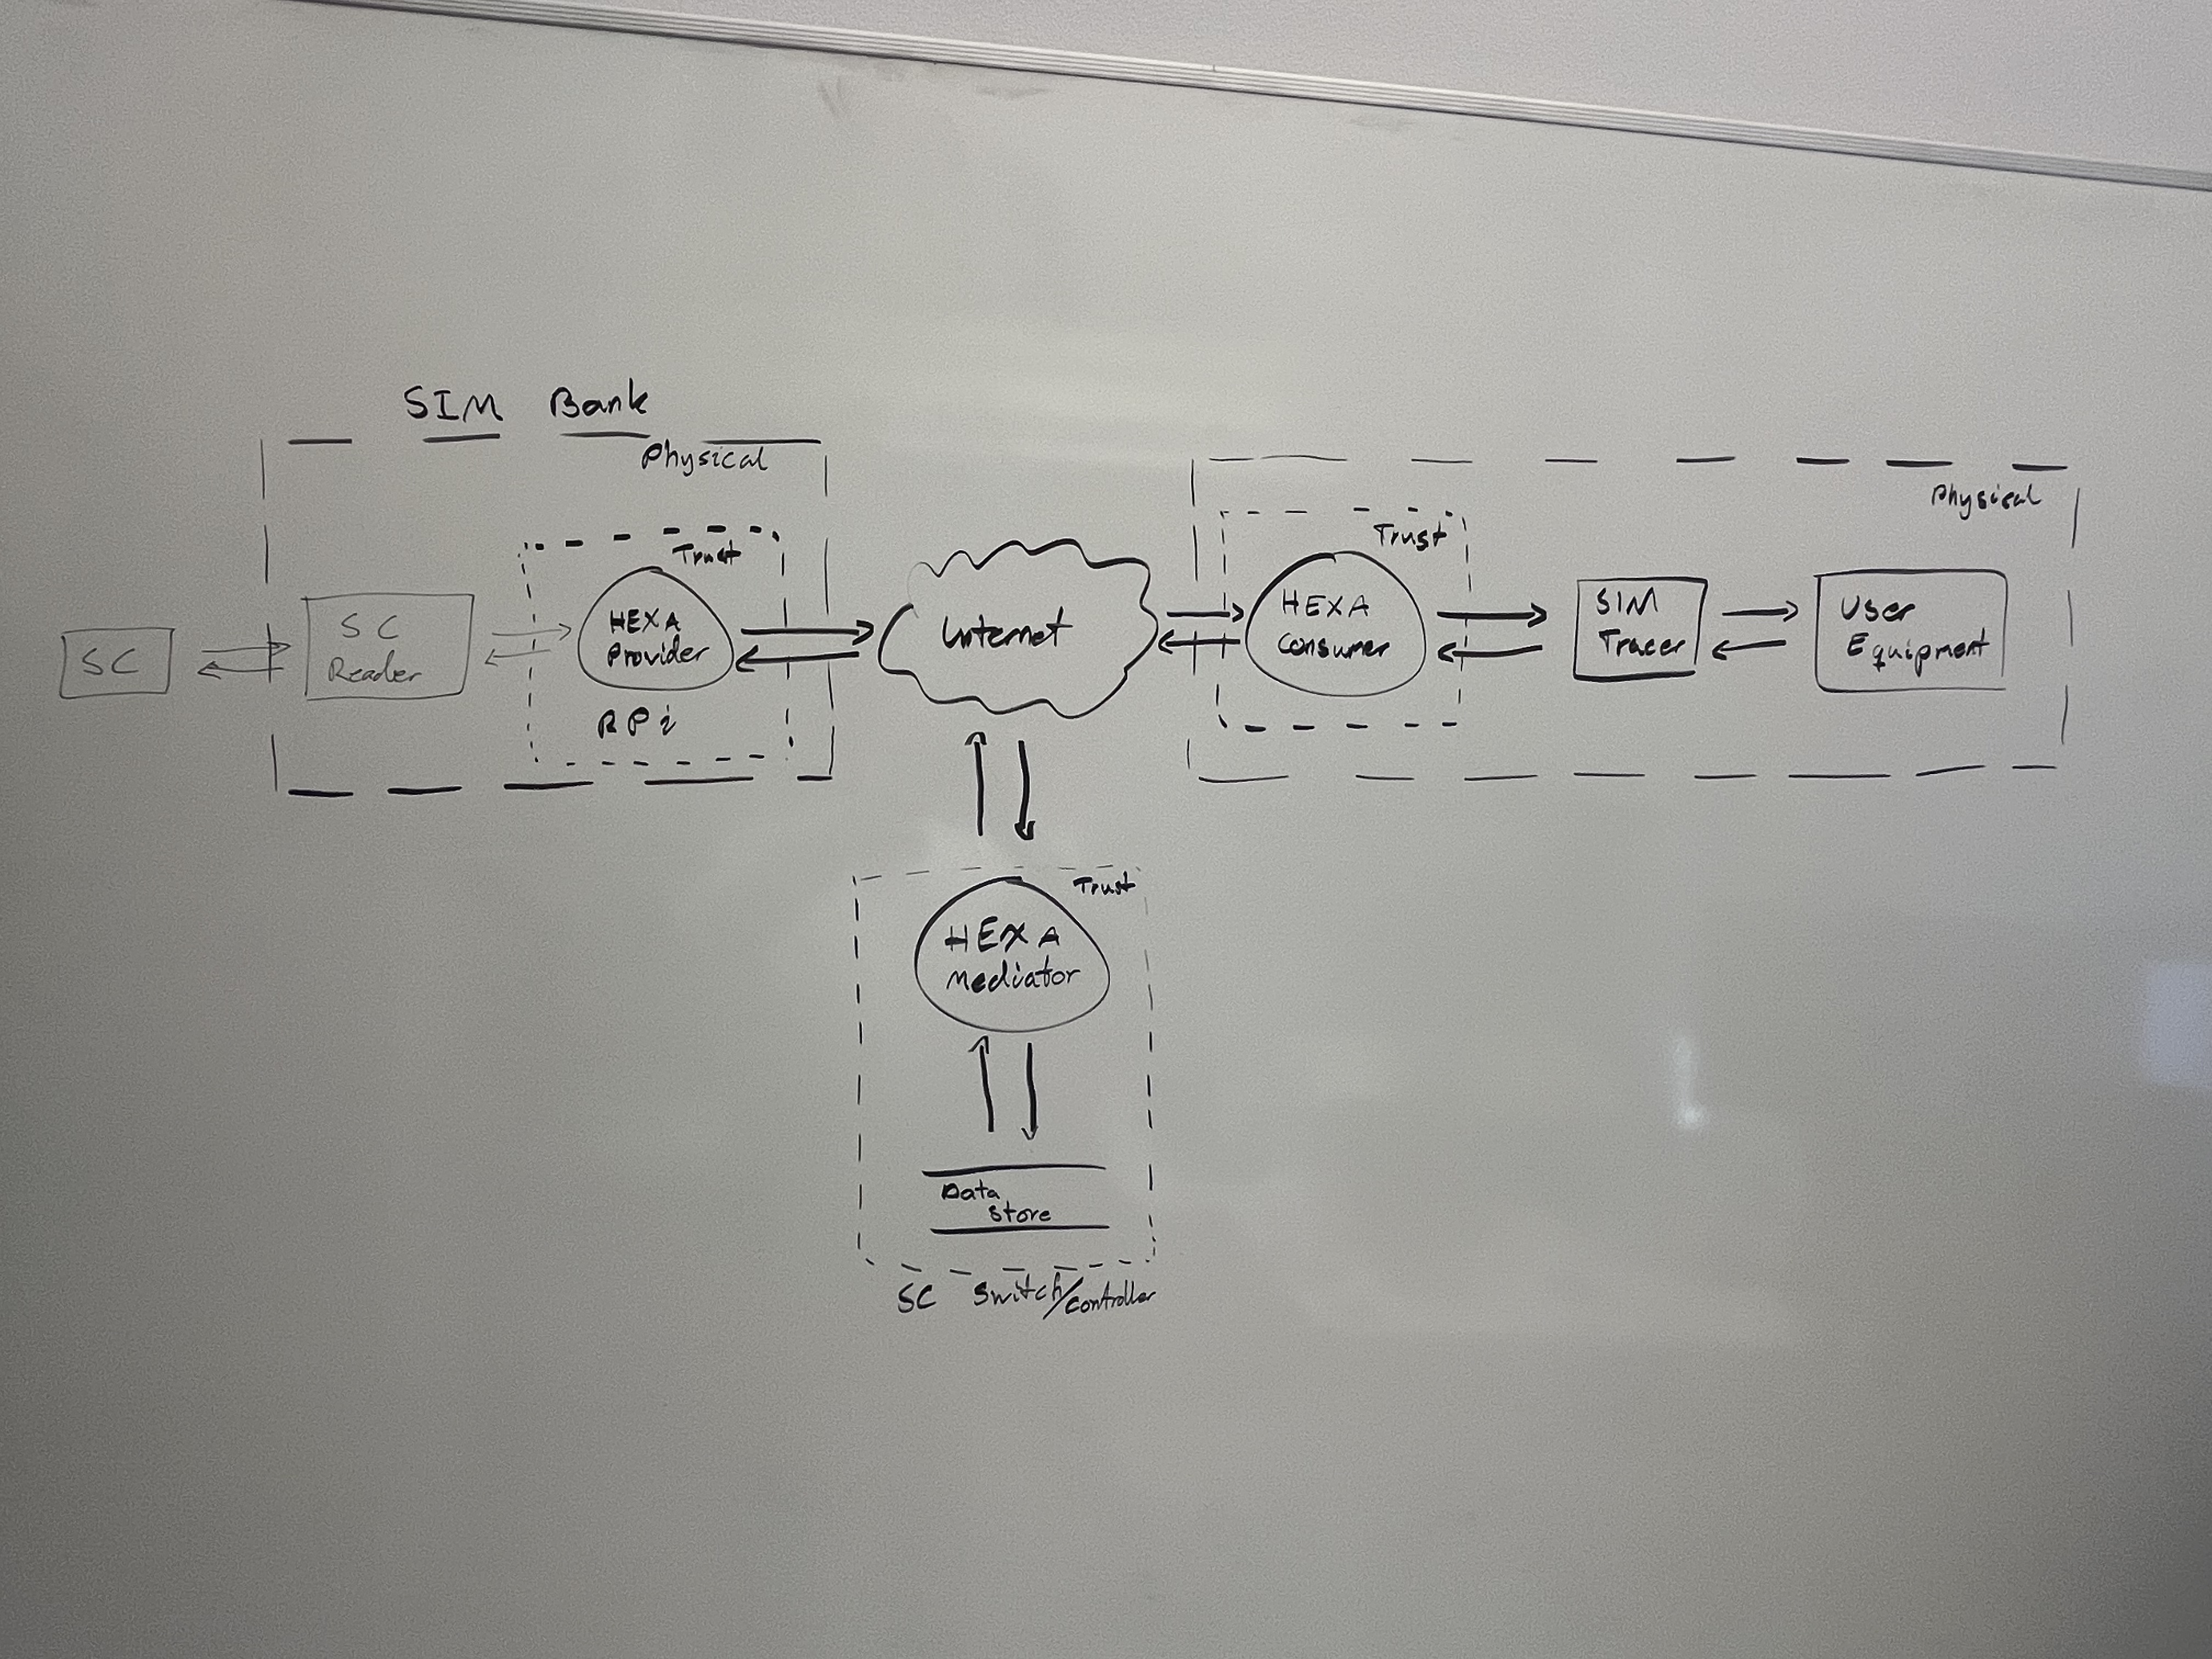
\includegraphics[width=0.9\textwidth]{images/dfd}
    \caption{(Temporary figure) A Data-flow diagram for the HEXA system}
    \label{fig:dfd}
\end{figure}



\end{document}
